The first step in running any environmental model is defining your
domain.  This section will bring us through the steps and rational
behind those steps and how to use ArcGIS to define your grid.

Before we can run our \ac{ctm}, \acs{cmaq}, we first have to run other
models to prepare inputs for \acs{cmaq}.  These models process
meteorology, emissions and terrain topology; and these other models
sometime require their own domains.

We want to set up a domain encompassing the north eastern United
States with a resolution of of 36 km$^2$.  To do this, we must:
\begin{itemize}
	\item configure the projection we wish to use
	\item set up a domain to run our meteorology
	\item set up a domain for \acs{cmaq}
\end{itemize}

%\hl{make a nested domain an ``extra''}

\section{Domain Specifications}

We will use a \emph{Lambert Conic Conformal} grid projection in this exercise.
This is the projection most commonly used for \acs{cmaq}, though other
projections are supported.

The specific projection we would like to use is not provided by ArcGIS by
default, so we will have to create it.  See appendix \ref{defining_projection}
for instructions on how to implement the following projection.  (A projection
file is also available in the included materials, named
\file{proj\_lcc\_cmaq.prj})

%Actual [http://svn.pontus.cee.carleton.ca/svn/models/doc/domain/Toronto12/rpo_lambert_proj.prj projection file] is available [http://svn.pontus.cee.carleton.ca/svn/models/doc/domain/Toronto12/rpo_lambert_proj.prj here].

The grid specifics are:
\begin{itemize}
	%\item False Easting: \textbf{2736.0}
	%\item False Northing: \textbf{2088}
	\item False Easting: \textbf{0.0}
	\item False Northing: \textbf{0.0}
	\item Central Meridian: \textbf{-97.0}
	\item Standard\_Parallel\_1: \textbf{33}
	\item Standard\_Parallel\_2: \textbf{45}
	\item Latitude\_Of\_Origin: \textbf{40}
	\item Linear Unit: \textbf{Kilometre}
\end{itemize}

Or, if you prefer the information in the standard \textbf{proj} format.
%+proj=lcc +datum=WGS84 +no_defs +lon_0=-97 +lat_1=33 +lat_2=40 +lat_0=40 +units=km +x_0=2736 +y_0=2088 +title="\acs{cmaq} RPO-NA LCC Shifted"
\begin{minted}{text}
+proj=lcc +datum=WGS84 +no_defs +lon_0=-97 +lat_1=33 +lat_2=40 +lat_0=40
   +units=km +x_0=0 +y_0=0 +title="\acs{cmaq} RPO-NA LCC"
\end{minted}
Though ArcGIS does display projection information in this form, it
is rather hidden.  Other GIS packages however (such as QGIS) use this
format more prominently.

%Note that we have named this domain ``shifted'', this is because we are
%including false easting and northings that we do not actually need for the
%projection (and will remove later.)  We are including these because they will
%make it easier to define our grids.  The false easting and northing in this
%setup actually defines the origin of our the \acs{cmaq} domain we are setting
%up.  We could just as easily remove the false easting and northing

Our \ac{cmaq} grid specification is:
\begin{itemize}
	\item A 36 km$^2$ spanning the North Eastern US.
	\item Grid origin (lower left corner) at: $(936, -576) \text{ km}$
	\item 44 rows, 40 columns.
\end{itemize}

This grid was chosen because it is a standard grid used in the
\acs{cmaq} test case.  If you're choosing a new domain, you want to
take the following into consideration:
\begin{itemize}
	\item Is my domain large enough to properly model transport processes for the time period I intend to model?
	\item Do my boundaries exclude any major emission sources close to my boundaries? \ie, would expanding my domain by another cell include a major emission source that impacts my main area of interest?
	\item Is my domain an appropriate size and resolution to model the chemistry in my area of interest?
\end{itemize}

To accommodate this grid, our meteorology should be larger by 3
cells.  Having a larger meteorological domain is is standard practice in air
quality modelling, though whether it be 3 cells or some other number is the
modellers choice.  The reason for a larger meteorological domain is to reduce
the effect of the meteorological boundaries on the \ac{ctm} domain.  These
extra cells are later removed such that the meteorological domain matches the
grid domain.

Therefore, our meteorological domain should be:
\begin{itemize}
	\item A 36 km$^2$ encompassing our \ac{cmaq} domain with a padding of 3 cells
	\item Grid origin (lower left corner) at: $(828, -684) \text{ km}$
	\item 50 rows, 46 columns.
\end{itemize}

\section{Drawing your domains in ArcGIS}
\label{drawing_domains}

Though not necessary, designing your grid in a GIS application -
though slow - can be incredibly helpful to visualize your domain(s)
and ensure they are exactly what you think they are.  Without any
visualization, the user may define their domain simply mathematically.
\eg~Toronto is X km away from our grid centre in our projection, our
cell size is Y, we want Z cells to be processed before Toronto, so we
need K cells.

The mathematical methods work of course, but become complicated when entering
domains into the different models.  For example, \acs{wrf}, a common
meteorological model, uses grid points rather than grid cells, and calculates
the offsets from the grid origin.  Meanwhile, \acs{cmaq}, our \acs{ctm}, uses
grid cells and requires inputs from the projection centre.

First, for context, add a shapefile for the continental US.  Such a
shape file can be downloaded at the Global Administrative Regions
website ( \url{http://www.gadm.org/} ) I recommend adding the
\file{USA\_adm1} file as it contains all the state boundaries.

We will use the \emph{Fishnet} tool to draw the grids onto your
projection to reduce the amount of confusion.  Though ArcGIS has a
native Fishnet tool, it is - in my opinion - less than intuitive to
use.  Therefore, this lesson recommends downloading a third-party
fishnet tool from
\url{http://arcscripts.esri.com/details.asp?dbid=12807}.  Once you
download this tool, add it to your menu bar, it should appear as in
figure \ref{fig:fishnet}.

\begin{figure}
	\centering
	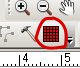
\includegraphics[width=0.10\textwidth]{fishnettool.jpg}
	\caption{Third-party Fishnet tool}
	\label{fig:fishnet}
\end{figure}

Use the fishnet tool to create the \acs{cmaq} domain specified above, \ie
\begin{itemize}
	\item X (km): \textbf{936}, Y (km): \textbf{-576}
	\item Rows: \textbf{44}, Cols: \textbf{40}
	\item Size of each Cell: \textbf{36}, \textbf{36}
	\item Specify Output Shapefile: \acs{cmaq}\_36
	\item Coordinate System (optional): Select the projection you created earlier
\end{itemize}

You should now see a new grid layer added.  At this point, I normally change it's colour to ``hallow" with a blue line colour.

Next, we want to create the meteorological domain.

\begin{itemize}
	\item X (km): \textbf{828}, Y (km): \textbf{-684}
	\item Rows: \textbf{50}, Cols: \textbf{46}
	\item Size of each Cell: \textbf{36}, \textbf{36}
	\item Specify Output Shapefile: \acs{wrf}\_36
	\item Coordinate System (optional): Import the projection off the previous grid
\end{itemize}

\begin{figure}
	\centering
	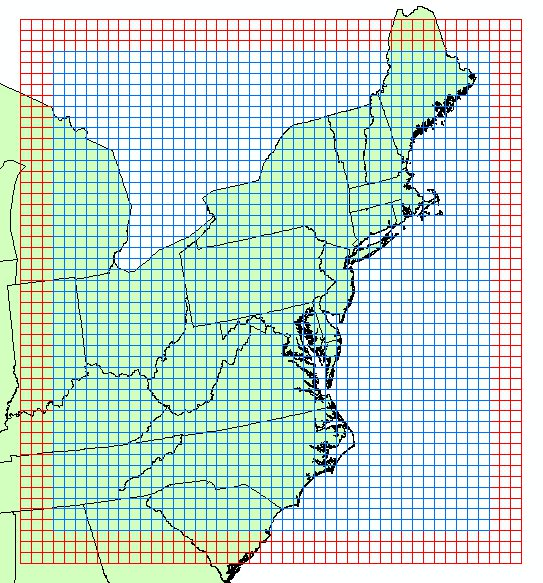
\includegraphics[width=0.60\textwidth]{grid_setup.jpg}
	\caption{Meteorological (red) and \acs{ctm} (blue) domain}
	\label{grid_setup}
\end{figure}

The specifics of setting up the models to run this domain, and running the models is outside the scope of this tutorial.

